%%%%%%%%%%%%%%%%%%%%%%%%%%%%%%%%%%%%%%%%%%%%%%%%%%%%%%%%%%%%%%%%%%
%%%%%%%%%%%%%%%%%%%%%%%%%%%%%%%%%%%%%%%%%%%%%%%%%%%%%%%%%%%%%%%%%%
%Packages
\documentclass[10pt, a4paper]{article}
\usepackage[top=3cm, bottom=4cm, left=3.5cm, right=3.5cm]{geometry}
\usepackage{amsmath,amsthm,amsfonts,amssymb,amscd, fancyhdr, color, comment, graphicx, environ}
\usepackage{float}
\usepackage{mathrsfs}
\usepackage[math-style=ISO]{unicode-math}
\setmathfont{Calibri}
\usepackage{lastpage}
\usepackage[dvipsnames]{xcolor}
\usepackage[framemethod=TikZ]{mdframed}
\usepackage{enumerate}
\usepackage[shortlabels]{enumitem}
\usepackage{fancyhdr}
\usepackage{indentfirst}
\usepackage{listings}
\usepackage{sectsty}
\usepackage{thmtools}
\usepackage{shadethm}
\usepackage{hyperref}
\usepackage{setspace}
\usepackage{biblatex}
\usepackage{csvsimple}
\usepackage{amsmath}
\usepackage{fontspec}
\usepackage{adjustbox}
\newfontfamily\faFont[Script=Arabic]{Calibri}   
\usepackage{bidi}
\newenvironment{Fa}{\begin{RTL}\faFont}{\end{RTL}}
\newcommand{\fa}[1]{{\faFont\RL{#1}}}
\hypersetup{
    colorlinks=true,
    linkcolor=blue,
    filecolor=magenta,      
    urlcolor=blue,
}
%%%%%%%%%%%%%%%%%%%%%%%%%%%%%%%%%%%%%%%%%%%%%%%%%%%%%%%%%%%%%%%%%%
%%%%%%%%%%%%%%%%%%%%%%%%%%%%%%%%%%%%%%%%%%%%%%%%%%%%%%%%%%%%%%%%%%
%Environment setup
\mdfsetup{skipabove=\topskip,skipbelow=\topskip}
\newrobustcmd\ExampleText{%
An \textit{inhomogeneous linear} differential equation has the form
\begin{align}
L[v ] = f,
\end{align}
where $L$ is a linear differential operator, $v$ is the dependent
variable, and $f$ is a given non−zero function of the independent
variables alone.
}
\mdfdefinestyle{theoremstyle}{%
linecolor=black,linewidth=1pt,%
frametitlerule=true,%
frametitlebackgroundcolor=gray!20,
innertopmargin=\topskip,
}
\mdtheorem[style=theoremstyle]{Problem}{Problem}
\newenvironment{Solution}{\textbf{Solution.}}

\definecolor{codegreen}{rgb}{0,0.6,0}
\definecolor{codegray}{rgb}{0.5,0.5,0.5}
\definecolor{codepurple}{rgb}{0.58,0,0.82}
\definecolor{backcolour}{rgb}{0.95,0.95,0.92}

\lstdefinestyle{mystyle}{
    backgroundcolor=\color{backcolour},   
    commentstyle=\color{codegreen},
    keywordstyle=\color{magenta},
    numberstyle=\tiny\color{codegray},
    stringstyle=\color{codepurple},
    basicstyle=\ttfamily\footnotesize,
    breakatwhitespace=false,         
    breaklines=true,                 
    captionpos=b,                    
    keepspaces=true,                 
    numbers=left,                    
    numbersep=5pt,                  
    showspaces=false,                
    showstringspaces=false,
    showtabs=false,                  
    tabsize=2
}

\lstset{style=mystyle}
%%%%%%%%%%%%%%%%%%%%%%%%%%%%%%%%%%%%%%%%%%%%%%%%%%%%%%%%%%%%%%%%%%
%%%%%%%%%%%%%%%%%%%%%%%%%%%%%%%%%%%%%%%%%%%%%%%%%%%%%%%%%%%%%%%%%%
%Fill in the appropriate information below
\newcommand{\norm}[1]{\left\lVert#1\right\rVert}     
\newcommand\course{NLP}                            % <-- course name   
\newcommand\hwnumber{1}                                 % <-- homework number
\newcommand\Information{Mohammadjavad Mehditabar - 98522049}                        % <-- personal information
%%%%%%%%%%%%%%%%%%%%%%%%%%%%%%%%%%%%%%%%%%%%%%%%%%%%%%%%%%%%%%%%%%
%%%%%%%%%%%%%%%%%%%%%%%%%%%%%%%%%%%%%%%%%%%%%%%%%%%%%%%%%%%%%%%%%%
%Page setup
\pagestyle{fancy}
\headheight 35pt
\lhead{\today}
\rhead{
\includegraphics[width=1cm]{images/iust-logo.png}}
\lfoot{}
\pagenumbering{arabic}
\cfoot{\small\thepage}
\rfoot{}
\headsep 1.2em
\renewcommand{\baselinestretch}{1.25}
%%%%%%%%%%%%%%%%%%%%%%%%%%%%%%%%%%%%%%%%%%%%%%%%%%%%%%%%%%%%%%%%%%
%%%%%%%%%%%%%%%%%%%%%%%%%%%%%%%%%%%%%%%%%%%%%%%%%%%%%%%%%%%%%%%%%%
%Add new commands here
% \renewcommand{\labelenumi}{\alph{enumi})}
\newcommand{\Z}{\mathbb Z}
\newcommand{\R}{\mathbb R}
\newcommand{\Q}{\mathbb Q}
\newcommand{\NN}{\mathbb N}
\newcommand{\PP}{\mathbb P}
\DeclareMathOperator{\Mod}{Mod} 
\renewcommand\lstlistingname{Algorithm}
\renewcommand\lstlistlistingname{Algorithms}
\def\lstlistingautorefname{Alg.}
\newtheorem*{theorem}{Theorem}
\newtheorem*{lemma}{Lemma}
\newtheorem{case}{Case}
\newcommand{\assign}{:=}
\newcommand{\infixiff}{\text{ iff }}
\newcommand{\nobracket}{}
\newcommand{\backassign}{=:}
\newcommand{\tmmathbf}[1]{\ensuremath{\boldsymbol{#1}}}
\newcommand{\tmop}[1]{\ensuremath{\operatorname{#1}}}
\newcommand{\tmtextbf}[1]{\text{{\bfseries{#1}}}}
\newcommand{\tmtextit}[1]{\text{{\itshape{#1}}}}

\newenvironment{itemizedot}{\begin{itemize} \renewcommand{\labelitemi}{$\bullet$}\renewcommand{\labelitemii}{$\bullet$}\renewcommand{\labelitemiii}{$\bullet$}\renewcommand{\labelitemiv}{$\bullet$}}{\end{itemize}}
\catcode`\<=\active \def<{
\fontencoding{T1}\selectfont\symbol{60}\fontencoding{\encodingdefault}}
\catcode`\>=\active \def>{
\fontencoding{T1}\selectfont\symbol{62}\fontencoding{\encodingdefault}}
\catcode`\<=\active \def<{
\fontencoding{T1}\selectfont\symbol{60}\fontencoding{\encodingdefault}}

%%%%%%%%%%%%%%%%%%%%%%%%%%%%%%%%%%%%%%%%%%%%%%%%%%%%%%%%%%%%%%%%%%
%%%%%%%%%%%%%%%%%%%%%%%%%%%%%%%%%%%%%%%%%%%%%%%%%%%%%%%%%%%%%%%%%%
%Begin now!



\begin{document}

\begin{titlepage}
    \begin{center}
        \vspace*{3cm}

        \Huge
        \textbf{Personality Detection on Persian Dataset}

        \vspace{1cm}
        \huge
        Phase \hwnumber

        \vspace{1.5cm}
        \Large

        \textbf{\Information}                      % <-- author


        \vfill

        \course \ Phase \hwnumber

        \vspace{1cm}

        
\includegraphics[width=0.4\textwidth]{images/iust-logo.png}
        \\

        \Large

        \today

    \end{center}
\end{titlepage}

%%%%%%%%%%%%%%%%%%%%%%%%%%%%%%%%%%%%%%%%%%%%%%%%%%%%%%%%%%%%%%%%%%
%%%%%%%%%%%%%%%%%%%%%%%%%%%%%%%%%%%%%%%%%%%%%%%%%%%%%%%%%%%%%%%%%%
%Start the assignment now
%%%%%%%%%%%%%%%%%%%%%%%%%%%%%%%%%%%%%%%%%%%%%%%%%%%%%%%%%%%%%%%%%%
%New problem
\newpage

\vspace*{0.1cm}

\tableofcontents

\newpage
% \vspace*{1pt}
\section{Data Overview}
Due to the lack of Persian datasets in the personality detection
field, gathering data from an adequate source is the main part of
our research. We came up with the idea of collecting data from
publicly available sources, thanks to social media, which is the best
and most applicable source. Because it contains a variety of people
and has a wide range of data, which is useful for us to collect. As a
result, we decided to choose Twitter as our data origin due to its
popularity, accessibility, and also comprise a lot of texts. We have
reached three different methods of collecting data

\section{Data Processing}

\subsection{Bio Search}

this dataset contains Iranian users with specified MBTI type of themselves in their bio.
There were some difficulties in distinguishing the language of some bios.
Hence they were solved by manual checking and some consideration of the Persian language.
Labels of this data are based on mentioned types in their bio, which we recognized by searching 16 MBTI types in their bio and automatically detecting them.
\\
This dataset consists of users' publicly available tweets and MBTI labels.
Figure \ref{bio_figure} shows a sample of our collected data based on a mentioned MBTI type on their bio.
\begin{figure}[h]
    \centering
    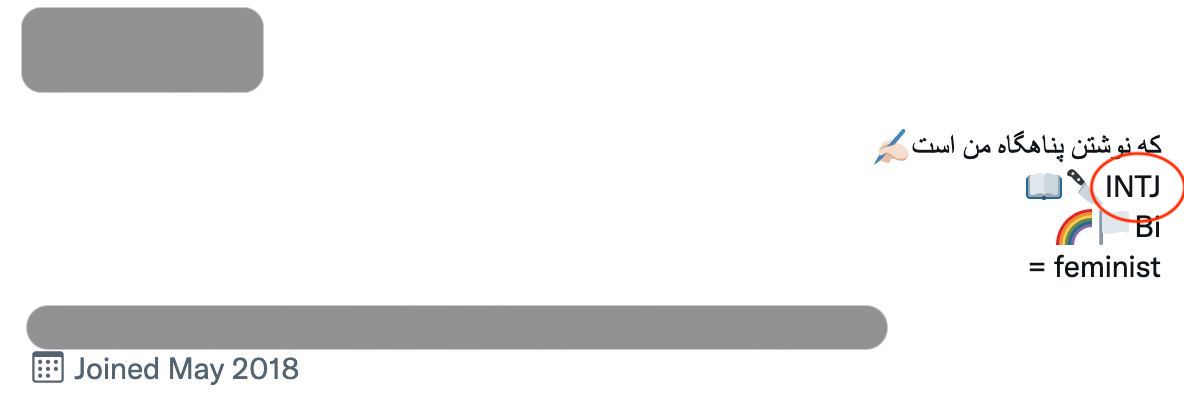
\includegraphics[width=.95\columnwidth]{images/sample.jpg}
    \caption{A sample of bio search}
    \label{bio_figure}
\end{figure}


\subsection{Tweet Search}
In this method, we tried collecting user tweets using a Python library called Twint.
Through this approach, we have searched for 16 possible MBTI labels in users' tweets in which one of these labels is mentioned.
Note that queried tweets are based on recent tweets in the Persian language.
We noticed that The type users mentioned in their tweets, may be irrelevant to themselves,
or they're saying some fact about this personality type or mentioning someone else's type.
Moreover, after filtering those users, we performed some elimination in a total separate step for the users
who have assigned themselves to multiple MBTI types. So these users are absolutely invalid for our dataset.
Hence there are chances that auto labeling makes a mistake in finding the correct label,
thus users are labeled manually so that ambiguity will be resolved.
\\
This dataset contains the gender of the user besides their tweets and MBTI label.
Figure \ref{tweet_figure} shows a sample of our collected data based on a mentioned MBTI type on their tweet.

\begin{figure}[h]
    \centering
    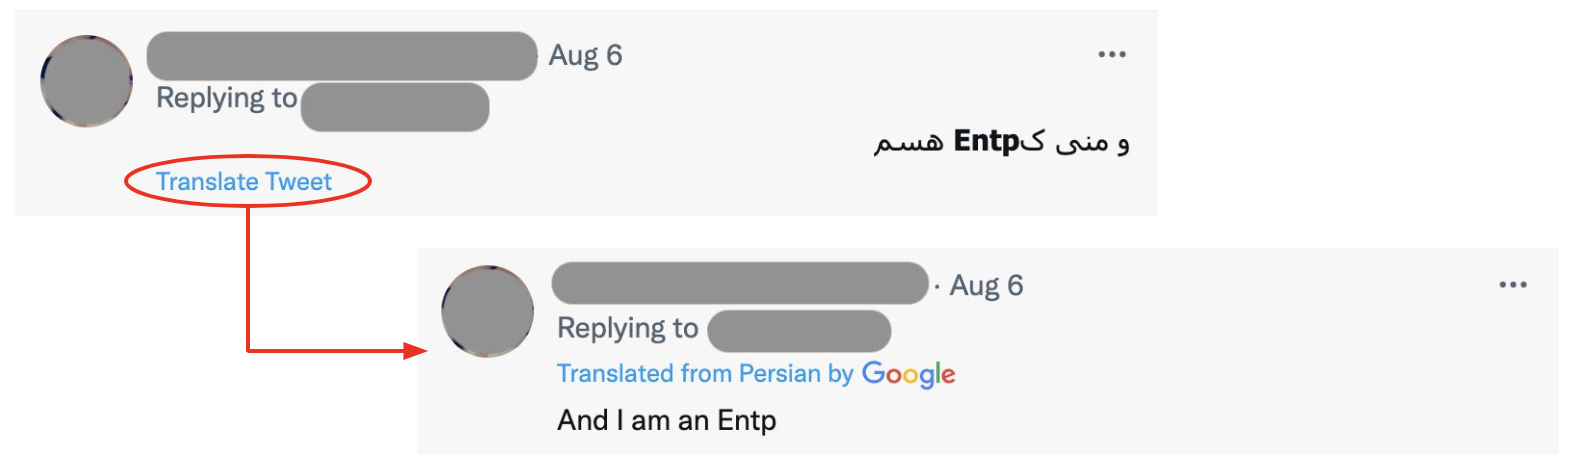
\includegraphics[width=.95\columnwidth]{images/sample-tweet.png}
    \caption{A sample of tweet search}
    \label{tweet_figure}
\end{figure}

\subsection{Questionnaire}
As our last method, we used a questionnaire to obtain more accurate data.
We can consider this data as the golden data.
The questionnaire was implemented in a web platform service with 60 standard well-known MBTI tests in which users
filled their Twitter IDs and answered those questions. We received a
few more data from users as well as their gender, location, degree of education,
and age for analyzing and adding more features to our data to perform well on the dataset.
Labeling them was based on their answer and how close they were to each of four binary class types (i.e. I/E, S/N, T/F, P/J),
which were calculated after completing the questionnaire.
Tweets of them are collected by the Python library Tweepy, which is a helpful tool to gain all their tweets.
Users are verified through the unique token generated for each user.
With this technique, we'll prevent fake data from entering our dataset.
Also, we filtered users to have at least 150 tweets, and their account is public.
Our questionnaire was utterly ethical since all users completed it voluntarily, and their account was public.

\subsection{Data Cleaning}
We follow a relatively straightforward strategy to clean our textual data.
Firstly, we find and replace some special patterns with unique tokens using regular expressions.
More specifically, we replace URLs with [LINK], usernames with [USERNAME], emojis with [EMOJI], and smileys with [SMILEY].
We also take a step further to filter out non-Persian characters.
For this purpose, we carefully select specific ranges of the Unicode characters to be allowed in our data.
We find that this step substantially improves the performance of our models.
Finally, we only preserve users that have more than 100 tweets after performing the above-mentioned cleanings.
\\
Also I should mention that, we used another approach which is cleaning more agressively. In this method we remove any non-Persian
characters and all tweets are splitted with just space, not any other punctuation marks. Currently we are using this method.
\\
After removing not-qualified users which were about 4356, we've got 3876 users at the end.

\section{Data Format}

\subsection{Folder Structure}
Data folder contains four subfolders. explaination of each folder :
\begin{itemize}
    \item raw : this also contains one subfolder and one json file:
          \begin{itemize}
              \item crawled : this folder is the raw crawled data from twitter that contains all tweets of a user which mentioned
                    his/her MBTI type in one of tweets.
              \item datasets.json : this file is the json file which has every username, label and their related raw tweets(which later we can use pandas library to load json file)
          \end{itemize}
    \item clean : this also contains one subfolder and one json file:
          \begin{itemize}
              \item crawled : this folder is the cleaned crawled data from twitter that contains all tweets of a user which mentioned
                    his/her MBTI type in one of tweets.
              \item datasets.json : this file is the json file which has every username, label and their related cleaned tweets(which later we can use pandas library to load json file)
          \end{itemize}
    \item sentence broken : sentence broken json file which has 4 columns : username, tweets, label, sentence tokenized tweets with \textit{hazm} library
    \item word broken : word broken json file which has 4 columns : username, tweets, label, word tokenized tweets with \textit{hazm} library
\end{itemize}
src folder contains two subfolders. explaination of each folder :
\begin{itemize}
    \item data processing : this folder is 3 folder and one python file.
          \begin{itemize}
              \item data collection : this folder is main part of crawling. It works in this way that first collect MBTI keywords in \textit{collect\_keyword\_tweets.py} then after crawling that user
                    it will save them on a csv file. after that all tweets of each user are collected in \textit{specific\_user\_tweets.py} file. the \textit{script.py}
                    file use these two file to create our raw dataset.
              \item data cleaning : this has scrpit subfolder in it which will handle the data cleaning file with \textit{ptpd.exe} file with running \textit{script.py} file. There is another subfolder which is main part of cleaning that has been implemented in \textit{F\#}.
              \item tokenizing : this has script \textit{tokenizer.py} which will generate sentence tokenizer and word tokenizer with \textit{hazm} library.
              \item main.py : this script is the main part for processing the above folder mentioned and it will run with this command \textit{python main.py all}
          \end{itemize}
    \item data analyzing : this will generate some statistic about our dataset. which is in stats folder
\end{itemize}
stats folder contains files which are generated for analyzing our dataset with different criterion which is mainly comprised by \textit{csv, png and json} file.
\subsection{Label Independency}
As I mentioned we have 16 different MBTI label which are formed on top of four separate traits(i.e. I/E, S/N, T/F, P/J).
So each user has unique label which is among these 16 label. For example a user can be \textit{INTJ} or \textit{ESTP}.

\section{Labeling Explaination}
Since there is ambiguity in each tweets with specific MBTI keyword and we don't know what they're describing in the tweet we had to
label each user manually. if user was mentioning their type we would've collected that user with all of his/her tweets.
So If a user said \fa{و منی که ENTP هستم}.
our group labeled him/her as an ENTP type and collect all of his/her tweets.
And on the other hand if a user said \fa{تایپ شخصیتی ENTP واقعا عجیبه}.
this is not mentioning his/her type so we wouldn't pick this user.
\\
\subsection{Dataset Unit Label}
our unit of labeling is for every single user which were filtered previously, we've collected all of his/her tweets and their related
Label. So we train our model on users with all of their tweets to predict their personality type.

\section{Data Analyzing}
In this section we're going to some details about our datasets and its relevant labels.

\subsection{Main Part Counts}
The table below shows exact number of sentence, words, unique words and number of all rows in our dataset.
\\
\begin{adjustbox}{center}
    \csvautotabular{../stats/base_data_stats.csv}
\end{adjustbox}
\\
\subsection{Common and Not Common Words Count}
In this part there are two tables showing each pair of labels how many words are common and not.

\subsubsection{Common Count}
\begin{adjustbox}{max width=\textwidth,totalheight=2in}
    \csvautotabular{../stats/common_count.csv}
\end{adjustbox}
\begin{center}
    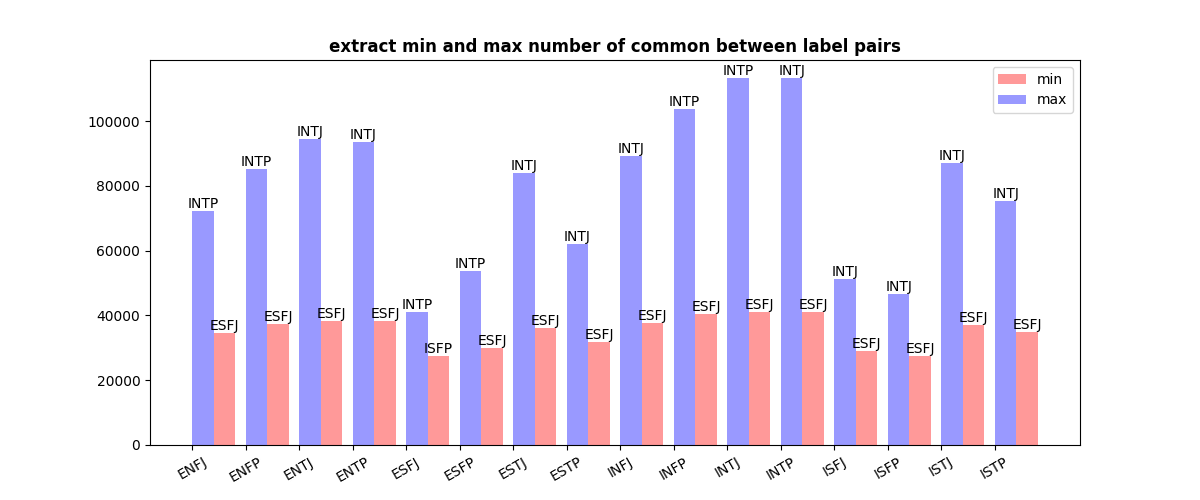
\includegraphics[width = \textwidth, height=2in]{../stats/common_count.png}
\end{center}

\subsubsection{Not Common Count}

\begin{adjustbox}{max width=\textwidth,totalheight=2in}
    \csvautotabular{../stats/not_common_count.csv}
\end{adjustbox}
\begin{center}
    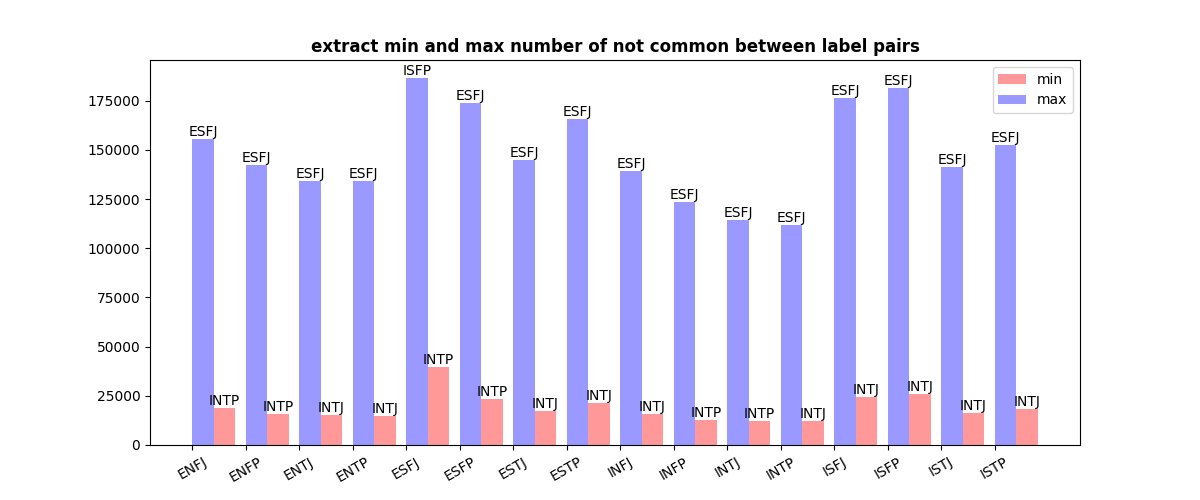
\includegraphics[width = \textwidth, height=2in]{../stats/not_common_count.png}
\end{center}

\subsection{Most Uncommon Between Label Pairs}
Since there are 16 MBTI labels and for computing most Uncommon words between every pair 16 X 16 = 256 so we can show tables but I showed them
in a sample image that is like below
\begin{figure}[H]
    \centering
    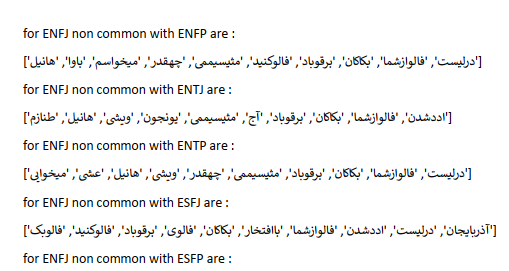
\includegraphics[width=0.7\linewidth]{../stats/most_uncommon_labels.png}
    \caption{most uncommon words between every 2 label}
\end{figure}

\subsection{Relative Normalized Frequency}
This criterion is also same as previous one that can't be fit in a page so I show some part of it
\begin{figure}[H]
    \centering
    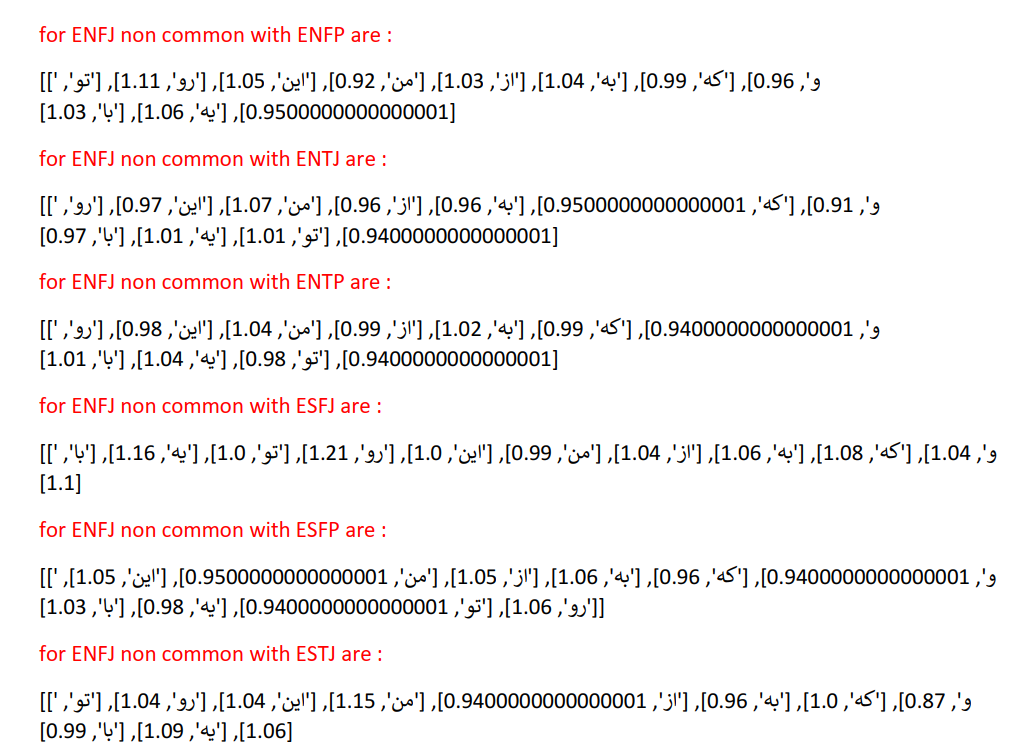
\includegraphics[width=0.7\linewidth]{../stats/RNF.png}
    \caption{RNF between every two pair}
\end{figure}
\newpage
\subsection{TF-IDF}
this is a criterion that computes text frequency in a document and inverse document frequency. The exact formula is in like this:
\begin{figure}[H]
    \begin{center}
        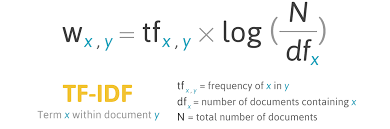
\includegraphics[width=0.8\linewidth]{images/tf-idf.png}
        \caption{tf-idf formula}
    \end{center}
\end{figure}
And according to the computation of above formula, results in the following table:
\\
\begin{Fa}
    \centering
    \begin{adjustbox}{max width=\textwidth,totalheight=6cm}
        \csvautotabular{../stats/tf-idf.csv}
    \end{adjustbox}
\end{Fa}
\vspace{2cm}
The above table shows tf-idf between every 2 pairs of label. and not suprisingly perposition words are in top occuring based on this criterion.
we see that the word \fa{"که"} happened more than any other perposition. And it seems in twitter Iranian use the word "very" so often that it'll be
translated to \fa{"خیلی"}. And the verb with most factor of tf-idf is \fa{"میشه"} that it's informal version of \fa{"می‌شود"}. and finally there is result that make
sense which I believe twitter users are more Intorvert as a result they should use more the word "me" in their tweets that its translation is \fa{"من"}. so these are
the facts that can be understood from the tf-idf table.
\newpage
\subsection{Unique Words Most And Least Frequent}
In this part we calculate which words happened the most and the least. For sake of fitting into the page
we just select first 30 of each part.
\begin{figure}[H]
    \begin{center}
        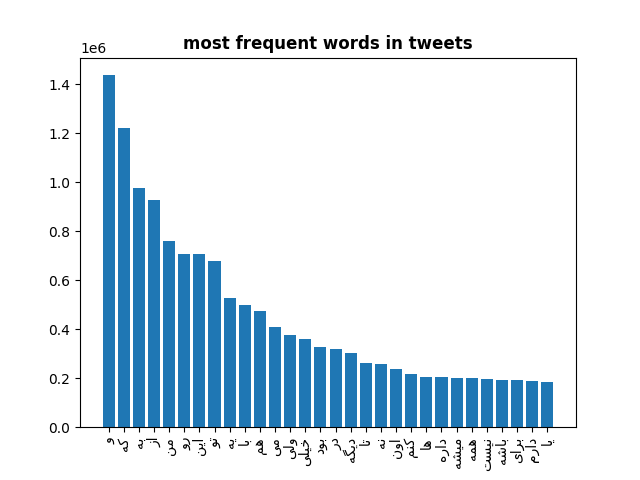
\includegraphics[width=0.6\linewidth]{../stats/most_frequent.png}
        \caption{Most Frequent Words}
    \end{center}
\end{figure}
\begin{figure}[H]
    \begin{center}
        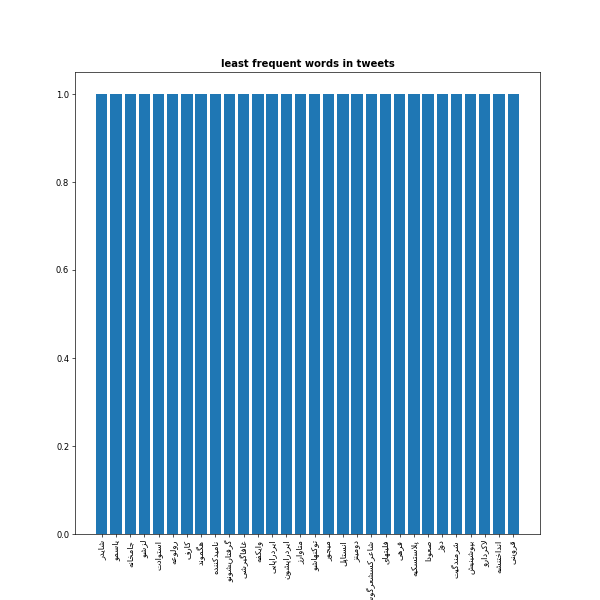
\includegraphics[width=0.6\linewidth]{../stats/least_frequent.png}
        \caption{Least Frequent Words}
    \end{center}
\end{figure}

Most occuring words are almost perposition and common verbs which happens to be around 1,4 milion. but for least frequent words all of them
are one.

\end{document}

